\chapter{Capture and Replay for Eiffel}
\section{Differences to Existing Implementation}
Selective capture and replay as described by Joshi and Orso \cite{orso05may} can not be directly applied to Eiffel. Although the core elements of the technique can be used in Eiffel, too, we need to adapt some parts. In this section the changes to the original implementation and reasons for these changes will be discussed.

\subsection{Language Aspects}
Even though Java and Eiffel are both object oriented languages, there are differences between these two languages, syntax left aside. Eiffel offers a wider set of language constructs, many times trying to solve problems inherently object oriented, whereas Java reused solutions from its ancestors, mainly C++. One example for this difference could be the Eiffel basic types, which can be treated as objects with methods and attributes versus the Java basic types, which are no objects. This section focuses on the differences between Java and Eiffel that influenced our implementation of selective capture and replay.

\subsubsection{Terminology} % diesen Titel weglassen?
Eiffel has a nomenclature that differs from other programming languages. Here the terminology is described according to \cite{oosc2} and compared to the one from Java.
\begin{center}
\begin{tabular}[]{|l|l|} \hline
 \textbf{Eiffel}&\textbf{Java} \\ \hline
 Attribute&Field \\ \hline
 Routine&Method \\ \hline
 Procedure&Method that has no return value \\ \hline
 Function&Method that has a return value \\ \hline
 Feature&Method or Attribute \\ \hline
\end{tabular} 
\end{center}

\subsubsection{Multiple Inheritance}
Eiffel is designed to support multiple inheritance, whereas in Java, only single inheritance is allowed. The original implementation assumes, that all subclasses of a class \emph{c} are in the observed set iff \emph{c} is also in the observed set. This makes it possible to statically decide whether an observed or an unobserved feature is accessed.

Translated to multiple inheritance, it would not be possible to have a class \emph{C} that inherits both from an observed class \emph{A} and an unobserved class \emph{B} (\figref{fig:obs_unobs_multiple_inheritance}).
\begin{figure}[ht]
  \centering
  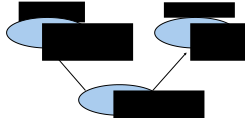
\includegraphics[width=0.5\textwidth]{illustrations/obs_unobs_multiple_inheritance}
  \caption{Conflict Due to Multiple Inheritance}
  \label{fig:obs_unobs_multiple_inheritance}
%\includegraphics{illustrations/capture_and_replay_generic_structure}
\end{figure}

Multiple inheritance is extensively used in Eiffel, thus this assumption would be too restrictive in our opinion. It would lead to big clusters that could not be divided into observed and unobserved set. 

Although Java does not allow multiple inheritance, it supports multiple interface inheritance. Joshi and Orso \cite{orso05may} mention that they need to dynamically determine if the target of an event is observed or unobserved in certain cases. We assume that multiple interface inheritance with a class that both implements an observed and unobserved interface  is at least one of these cases. They use the \texttt{instanceof} operator determine if an object is an instance of an observed class.

We will present a solution that always determines dynamically, if an object is an instance of an observed class (\emph{observed object}) or an instance of an unobserved class (\emph{unobserved object}), together with a proposal how to solve this problem without reflection.

\subsubsection{Read Only Attributes}
Eiffel strictly follows the \emph{uniform access principle} \cite{oosc2}. The principle states that it should not be visible to the clients whether features are implemented through storage or computation. This ensures that the implementation of a feature could be changed from attribute to function or vice versa. One of the consequences of this principle is that clients of a class cannot write to attributes, as they could be implemented as a function as well.

In Java, this principle is not ensured because clients of a class can write to their fields. For our implementation of selective capture and replay, this limits the events related to field accesses to OUTREAD. Both OUTWRITE and INWRITE can not happen, because write access to fields is restricted to their class, thus there can not be any write accesses to fields from observed to unobserved or reverse.

\subsection{Target Application}
As a first application that could use selective capture and replay in Eiffel, Cdd, a tool for Contract Driven Development \cite{cdd07} was chosen. Cdd allows programmers to extract test cases from failing program runs. The contracts that are present in the code are used as test oracles.Cdd is not always able to generate such a test case:

\begin{description}
\item [Prestate extraction:] The state before calling the failing feature (which is needed to generate a test case) is extracted using the state at the time of failure. Because not all instructions between feature call and failure can be undone, the extraction of the prestate is not always possible.
\item [Non-determinism:] If the failing feature reads values from sources that don't always return the same values (eg. user input), it's not generally possible to run the test cases with the same result as in the failing run.
\item [External state:] When the feature relies on state that is not stored in Eiffel objects (e.g. in C structs), Cdd is not able to gather this state for the test.
\end{description}

These limitations can be resolved using selective capture and replay:
\begin{description}
\item [Prestate extraction:] By setting a breakpoint at the beginning of the failing feature, it is possible to extract the prestate during the replay of the application.
\item [Non-determinism:] When adding all non-deterministic classes to the unobserved set, it can be ensured that the replay of the run is deterministic.
\item [External State:] All classes that wrap external state can be added to the unobserved set. Thus interactions with these classes can be replayed easily.
\end{description}

Prestate extraction using selective capture and replay requires an immediate rerun of the application under test. Because complete recompiles in Eiffel last for tens of minutes up to hours, we can not afford to instrument the application again before replaying it. Thus it is necessary to design the code instrumentation to be both applicable for capture and replay phase. We pushed this approach even further to allow the user to disable the whole instrumentation. This allows execution with minimal overhead if capture and replay is not needed without recompiling the application.

\section{Idea for Code Instrumentation}


%weitere Unterschiede:
% - creation procedures nicht gesondert instrumentiert --> synchronisierung bei outcalls. sonst muessten die unobserved Klassen nicht instrumentiert werden (nur outcallret) (?)

\section {Limitations}
%-Konstruktoren nach ANY exportiert (fehlende unterstuetzung von Eiffel-Seite fuer Konstruktoren)
%- Access modifiers e.g. export of a observed feature only to an unobserved class --> replay not possible.